% !TEX encoding = UTF-8
% !TEX TS-program = pdflatex
% !TEX root = ../Articolo.tex
% !TEX spellcheck = it-IT

%************************************************
\section{DEM Characterization Workflow Coarse Particles}
\label{section:Demcharacterizationworkflowcoarseparticles}
%************************************************

\subsection{Jenike's  Shear Cell tester}
\label{subsection:jenikeshearcell}

We have performed from 6 to 16 experiments per bulk material.\\

\subsubsection{SCT simulation}
\label{subsubsection:sctsimulation}

The script has been modified to run on 32 cores over $Mach$. As of now each shear cell experiment is simulated approx. 250 times with different combinations of parameters.
As can be seen in Fig. \ref{010dCylDpComparison}, a wall effect appears in the simulations, an the coefficient of internal friction decreases if the cell dimension grows. Since a bigger dimension means more particles and more computational demand, only a part of the simulations have been realized with a larger cell's diameter. The Neural Network, see section \ref{subsection:microparameters}, will account also for this $wall$ effect.\\
\begin{figure}[!h]
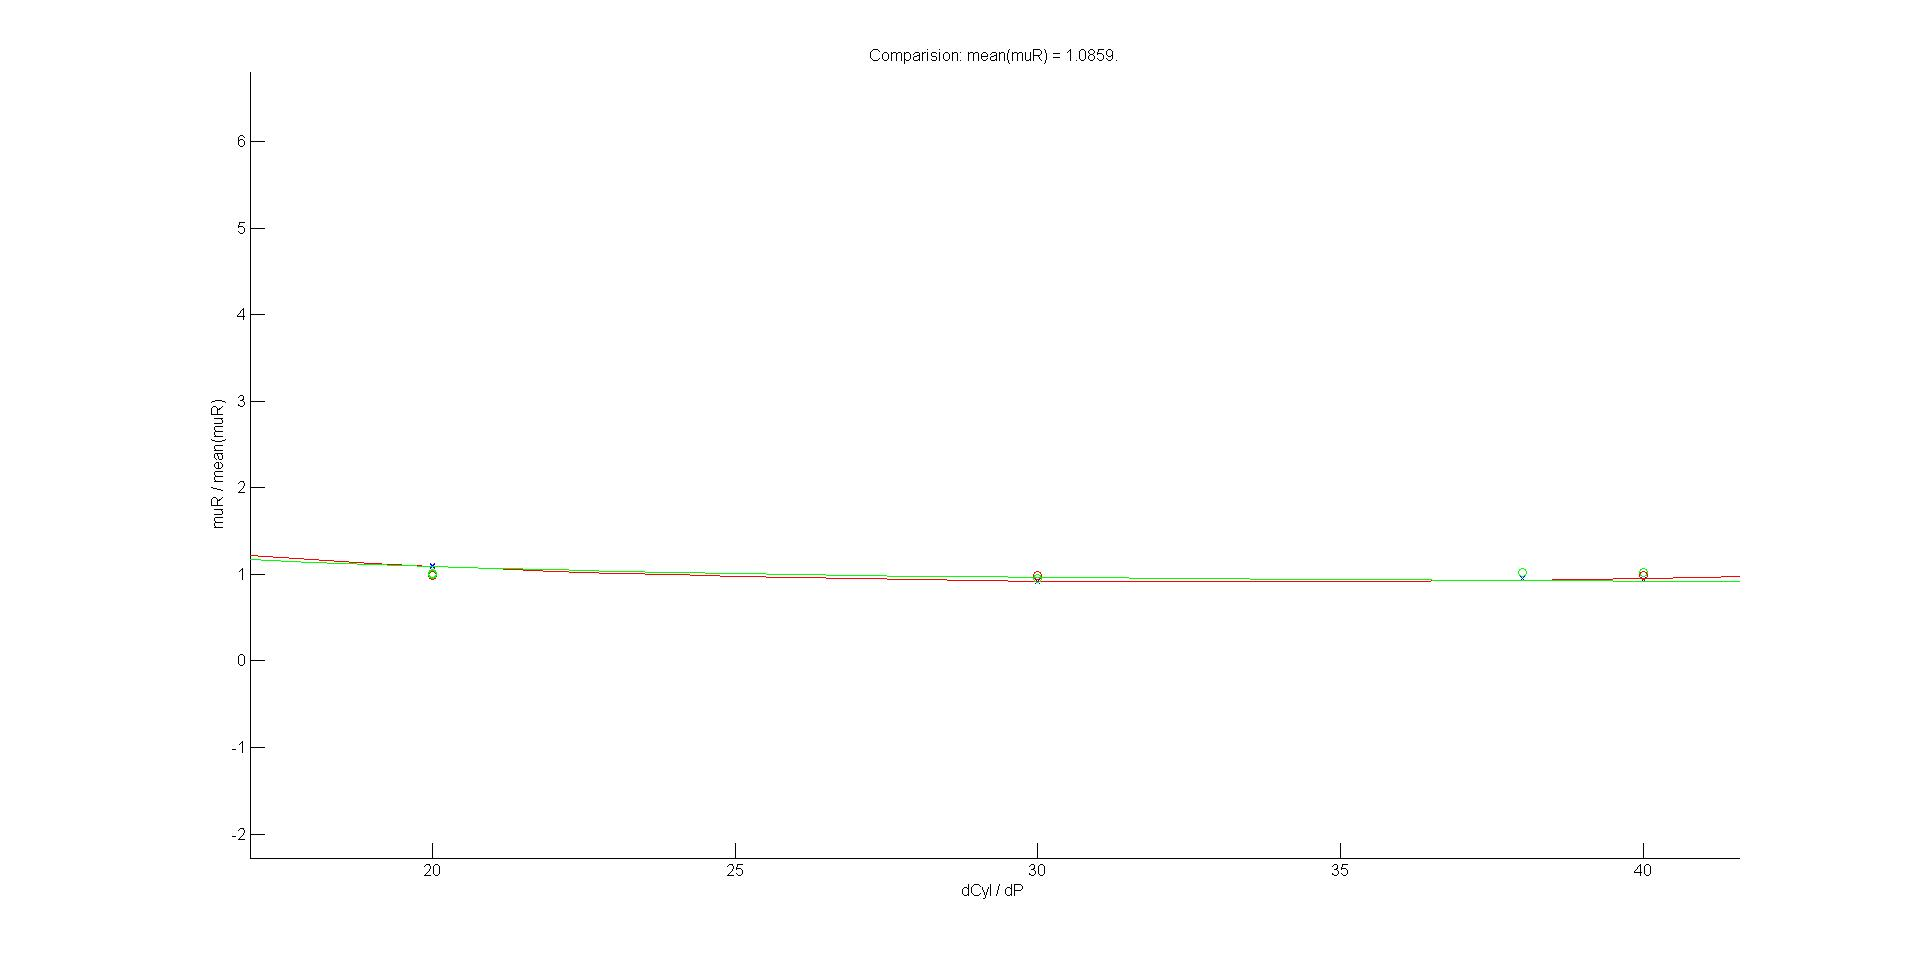
\includegraphics[width=.96\columnwidth]{010dCylDpComparison}
\caption{increased geometry effect}
\label{010dCylDpComparison}
\end{figure}

I received on the 10th of September this message from Mach: \textit{qsub: Maximum number of jobs for group k3b02 already in queue std.q}, with 35 scripts in queue (of them 14 are running, occupying 512 cores), when I tried to add a new script to the queue.
Now I have 18 scripts in queue (of them 7 are running, occupying 256 cores), but, since then, when I try to add a new script a receive the same error.
Since I am yet the only one in the department using Mach, I will contact the Administrator ASAP.\\

\subsection{Angle of Repose}
\label{subsection:aor}

For each bulk have been performed at least 2 experiments, of which the mean, median and variance values have been considered.\\

\subsubsection{AOR simulation}
\label{subsubsection:aorsimulation}

The script has been modified to run on 32 cores over $Mach$. As of now each material is simulated approx. 108 times with different combinations of parameters.\\

\subsection{Granulometric curves}
\label{subsection:granulometric curves}

I have completed sieving of all materials (except from 0 to 1.25 mm iron ore) and I have for them:
\begin{itemize}
\item{the granulometric curve;}
\item{the mean radius (R);}
\end{itemize}

\subsection{COR characterization}
\label{subsection:corcharacterization}

A new system based on frequency has been suggested. I will start working on it ASAP.

\subsection{Hollow spheres}
\label{subsection:hollowspheres}

This project will remain in stand-by until further notice.

\subsection{Rolling drum}
\label{subsection:rolling drum}

Both the experiment and the simulation manage to rotate the spheres at a given velocity.
To identify the slope in the middle of the experimental drum have been suggested:
\begin{itemize}
\item{to put a laser measurement system in the middle of the beam, that rotates together with the drum, but at least once per turn it registers correctly the slope's angle;}
\item{an "unstable" system connected to a load cell: when in a steady-state the load on the cell will be $0$, when in movement the load over the cell would allow to determine the mass of the "inclined" material;}
\end{itemize}
To identify the slope in the middle of the numerical drum I will work with LIGGGHTS $compute ~~ crosssection$.\\

I will proceed and complete ASAP with the documentation for all these experiments.\\


trotaculo